\chapter{Diskussion}
\label{sec:diskussion}

In diesem Abschnitt wird die Plausibilität der erhobenen Daten zur Analyse der Müllprobe 2 überprüft und diskutiert.\\ \\
\textcolor{red}{Carbonate nur Teil von TIC. TIC fehlt in der Betrachtung}\\
Beginnend mit dem Carbonatgehalt werden diese als wichtige Füll- und Zuschlagsstoffe für Papier, Pappe und diverse Kunststoffe eingesetzt. Für die untersuchte Müllprobe II fällt mit einem mittleren Carbonatgehalt von $\SI{5,3}{\mpercent}$ (siehe Abschnitt \ref{sec:tic}) dieser im Vergleich zu Carbonatgehalten für Papier mit bis zu $\SI{30}{\mpercent}$ \cite{Wikipedia.21.11.2019} und für Kunststoffe von $10 - \SI{50}{\mpercent}$ \cite{PolymerServiceGmbHMerseburg.13.08.2019} gering aus. Da aus der optischen Betrachtung des Mülls nicht nur Papier- und Kunststoffreste zu erkennen sind, sondern auch fasrige und \textbf{ veraschte} Komponenten, ist es durchaus plausibel, dass der Carbonatgehalt entsprechend kleiner ausfällt. \\
In diesem Versuch wurde der Carbonatgehalt für zwei Stichproben bestimmt, welche von einander eine Abweichung von 3\% aufweisen, was sich auf die inhomogene Zusammensetzung der Müllprobe selbst zurückführen lässt.\linebreak
Die Abweichungen bezüglich der Kalibrierkurve könnten sich ebenfalls auf diese Inhomogenität zurückführen lassen, jedoch wäre an dieser Stelle weitere Kalibrierpunkte, sowie weitere Messungen mit Müllproben sinnvoll, um repräsentative Aussagen treffen zu können. Nähere Infos zur Fehlerbetrachtung finden sich unter Abschnitt \ref{sec:fehler}.\\

\textcolor{red}{Muss mal noch schön mit eingebunden bzw. gekürzt werden}\\
\textcolor{blue}{\textit{Die wichtigste anorganische Kohlenstoffquelle in der Müllprobe sind vermutlich Carbonate.
Carbonate sind wichtige Füll- und Zuschlagsstoffe für Papier, Pappe und diverse Kunststoffe. Herkömmliches Papier kann dabei einen Füllstoffanteil von bis zu 30 \% \cite{Wikipedia.21.11.2019} aufweisen. Im Kunststoff PVC-U dient Calciumcarbonat unter anderem zur Steigerung der Schlagzähigkeit und der Oberflächengüte. Hart-PVC profitiert durch die Anhebung des E-Moduls, der Bruchdehnung, Schlagzähigkeit, Zugfestigkeit und des Oberflächenglanzes. Selbst die Wetterbeständigkeit verbessert sich. Bei vielen weiteren Kunststoffen ergibt sich durch die Zugabe von Calciumcarbonat neben einer Vielzahl von werkstofftechnischen Verbesserungen auch ein  entscheidender Preisvorteil. \cite{domininghausKunststoffeUndIhre1998}. Der Anteil reicht dabei von 3\% bis etwa 50\% Calciumcarbonat \cite{domininghausKunststoffeUndIhre1998}.\\
Die unbekannte Zusammensetzung der Müllprobe und die uneinheitliche Anwendung von Zuschlag- und Füllstoffen lassen kaum einen Vergleich mit anderen Proben zu. \\
In der Endkonsequenz könnte jeder Carbonatgehalt durch Füllstoffe erklärt werden. Ein weiterer Einflussfaktor sind Verunreinigungen. Teilweise werden anfallende Abfälle nicht korrekt getrennt. Ein wahrscheinliches Szenario wäre die Entsorgung nicht vollkommen restentleerter Kalksäcke. Die Säcke bestehen aus einer Kunststoffschicht und einer äußeren Papierhülle. Der enthaltene Kalk verfälscht die Messergebnisse. Ebenso könnte Kehricht im untersuchten Müll entsorgt worden sein.}}

\newpage

%Plausibilität TC
\textcolor{red}{Vergleich mit anderen Proben fehlt tab.\ref{tab:tc_messung}}\\
Der TC-Gehalt liegt laut dem \textit{Analysegerät} bei $\approx 27\%$ (siehe Tabelle \ref{tab:tc_messung}). Aufgrund der optischen Zusammensetzung des Mülls mit teilweise enthaltenen Papier, Pappe und Kunststoffschnipseln sowie den Textilfasern und ascheähnlichen Resten könnte der Kohlenstoffgehalt plausibel sein. Verglichen mit Tabelle \ref{tab:tc_vergleich} \cite[S.11]{HansGunterRamke.} scheint sich die Plausibilität mit den Daten für Feinmüll gemischt mit Pappe, Papier und Kunststoffen zu decken bzw. grob aufgerundet mit dem unteren Wert von Hausmüll mit \SI{30}{\percent}.\\
Für die Blindprobe und die vorbehandelte Probe durch die Bestimmung des TIC fallen andere Werte als die der Originalen Müllprobe an. Die ist aufgrund der unterschiedlichen Zusammensetzung aller drei Proben auch zu erwarten. Für die Blindprobe wäre, wenn es sich um reines \ce{CaCO3} gehandelt hätte ein Wert von \SI{12}{\mpercent} zu erwarten gewesen (siehe Gleichungen \ref{gl:3} und \ref{gl:4}). Da jedoch keine absolute Reinheit garantiert werden kann, fällt der Messwert entsprechend kleiner aus. Um die Plausibilität des Wertes der Blindprobe zu prüfen müssten an dieser Stelle weitere Informationen zur Reinheit der Blindprobe bekannt sein bzw. ermittelt werden, da dieser Wert um rund das 30-fache kleiner ausfällt, als für eine Reinstprobe.\\
Der Messwert für die vorbehandelte Probe durch die TIC-Bestimmung liegt bei \SI{4,39}{\mpercent}. Fälschlicherweise könnte man erwarten, dass dieser Wert, aufgrund des ausgetriebenen anorganischen Kohlenstoffs bei $\approx \SI{26}{\mpercent}$ liegen müsste. Da jedoch für das Austreiben der Carbonat Phosphorsäure und zur Neutralisation Natronlauge hinzugefügt wurde, verfälschen diese die Masse der Probe und man erhält somit einen anderen Messwert. Möglich wäre es an dieser Stelle die Masse der zugeführten Säure und Base einzubeziehen und somit einen neuen Messwert zu errechnen 
%Tabelle START
\vspace*{-3.5mm}
\renewcommand{\arraystretch}{1.2}
\begin{table}[h!]
	\centering
	\caption[Elementgehalte von Restabfall und ausgewählter Fraktionen]{Elementgehalte von Restabfall und ausgewählter Fraktionen \cite[S.11]{HansGunterRamke.}}
	\label{tab:tc_vergleich}
	\resizebox{15cm}{!}{
	\begin{tabulary}{1.2\textwidth}{L|CCCCC}
		\hline
		\textbf{Parameter}	& \mbox{\textbf{Hausmüll \, \,}} & \textbf{Fraktion A} \linebreak Papier, Pappe	& \textbf{Fraktion B} \linebreak Kunststoffe, etc.	& \textbf{Fraktion C} \linebreak Feinmüll & \textbf{Fraktion D} \linebreak Bioabfall\\
		\hline
		Kohlenstoff C  $ [TS\%] $ & 30-40&40&54&19&31\\
		Wasserstoff H  $ [TS\%] $ &4-5&6&8&3&4\\
		Stickstoff N  $ [TS\%] $ &0,3-0,5&0,3&0,9&0,4&2,1\\
		Sauerstoff O  $ [TS\%] $ &17-30&37&17&17&20\\
		\hline
	\end{tabulary}
}
\end{table}
\FloatBarrier
{\footnotesize \textbf{Fraktion A:} Papier, Pappe \quad \quad \quad \hspace*{0.7mm} \textbf{Fraktion B:} Kunststoffe, Holz, Leder, Textilien, Verbunde}\\
{\footnotesize \textbf{Fraktion C:} Feinmüll < 8 mm \quad \quad \textbf{Fraktion D:} Mittelmüll 8 – 40 mm, Vegetabilien}\\

Gegenüber anderer Untersuchungen ist der in diesem Versuch ermittelte Kohlenstoffgehalt eher niedrig \cite{Schwarzboeck2018}.

\textcolor{red}{Auf was genau in der Quelle beziehst du dich ? Seitenzahl, Tabelle oder so}. 

Die Müllprobe kommt einem Ersatzbrennstoff sehr nah. Darum die Ergebnisse mit Artikeln über selbige verglichen werden. 

\textcolor{red}{Verstehe den Satz nicht so ganz :/} \\

Die Feuchtigkeit in der Untersuchten Müllprobe kann praktisch nur im Papier und ähnlichem enthalten sein. Kunststoffe binden Feuchtigkeit praktisch nur als Anhaftung an ihrer Oberfläche \cite[S.3]{LLA_Abfallanalyse}. Der Müll fühlte sich trocken an und haftete auch nicht feuchtigkeitsbedingt zusammen.
Eine allgemeine Hausmüllprobe besitzt einen Wassergehalt von $\approx 35\%$  (siehe Abb. \ref{fig:ersatzbrennstoffe}). Vergleicht man die untersuchte Probe damit erscheint der berechnete Wert für den Wassergehalt als nicht plausibel. Da jedoch auch für Müllfraktionen wie Steine, Kunststoffe, Keramik, Verbundstoffe, etc. kein Wassergehalt in der Quelle (siehe Abb. \ref{fig:ersatzbrennstoffe}) angegeben ist, kann man darauf schließen, dass der Wassergehalt nur bei entsprechend hygroskopischen bzw. schon stark feuchten bis nassen Müllfraktionen berücksichtigt wird. Der Wassergehalt der Müllprobe fällt mit $\approx \SI{3}{\percent}$ als sehr gering aus und kann somit als nahezu "`trocken"' angenommen werden.\\
Der Unterschied im Wassergehalt zwischen der originalen Probe und der für die TIC-Analyse behandelten Probe lässt sich auf die zugegebene Phosphorsäure bzw. Natronlauge zurückführen. Dieser Wassergehalt gibt keine offensichtlich sinnvolle Information preis.

%Start
\begin{figure}[h!]
	\centering
	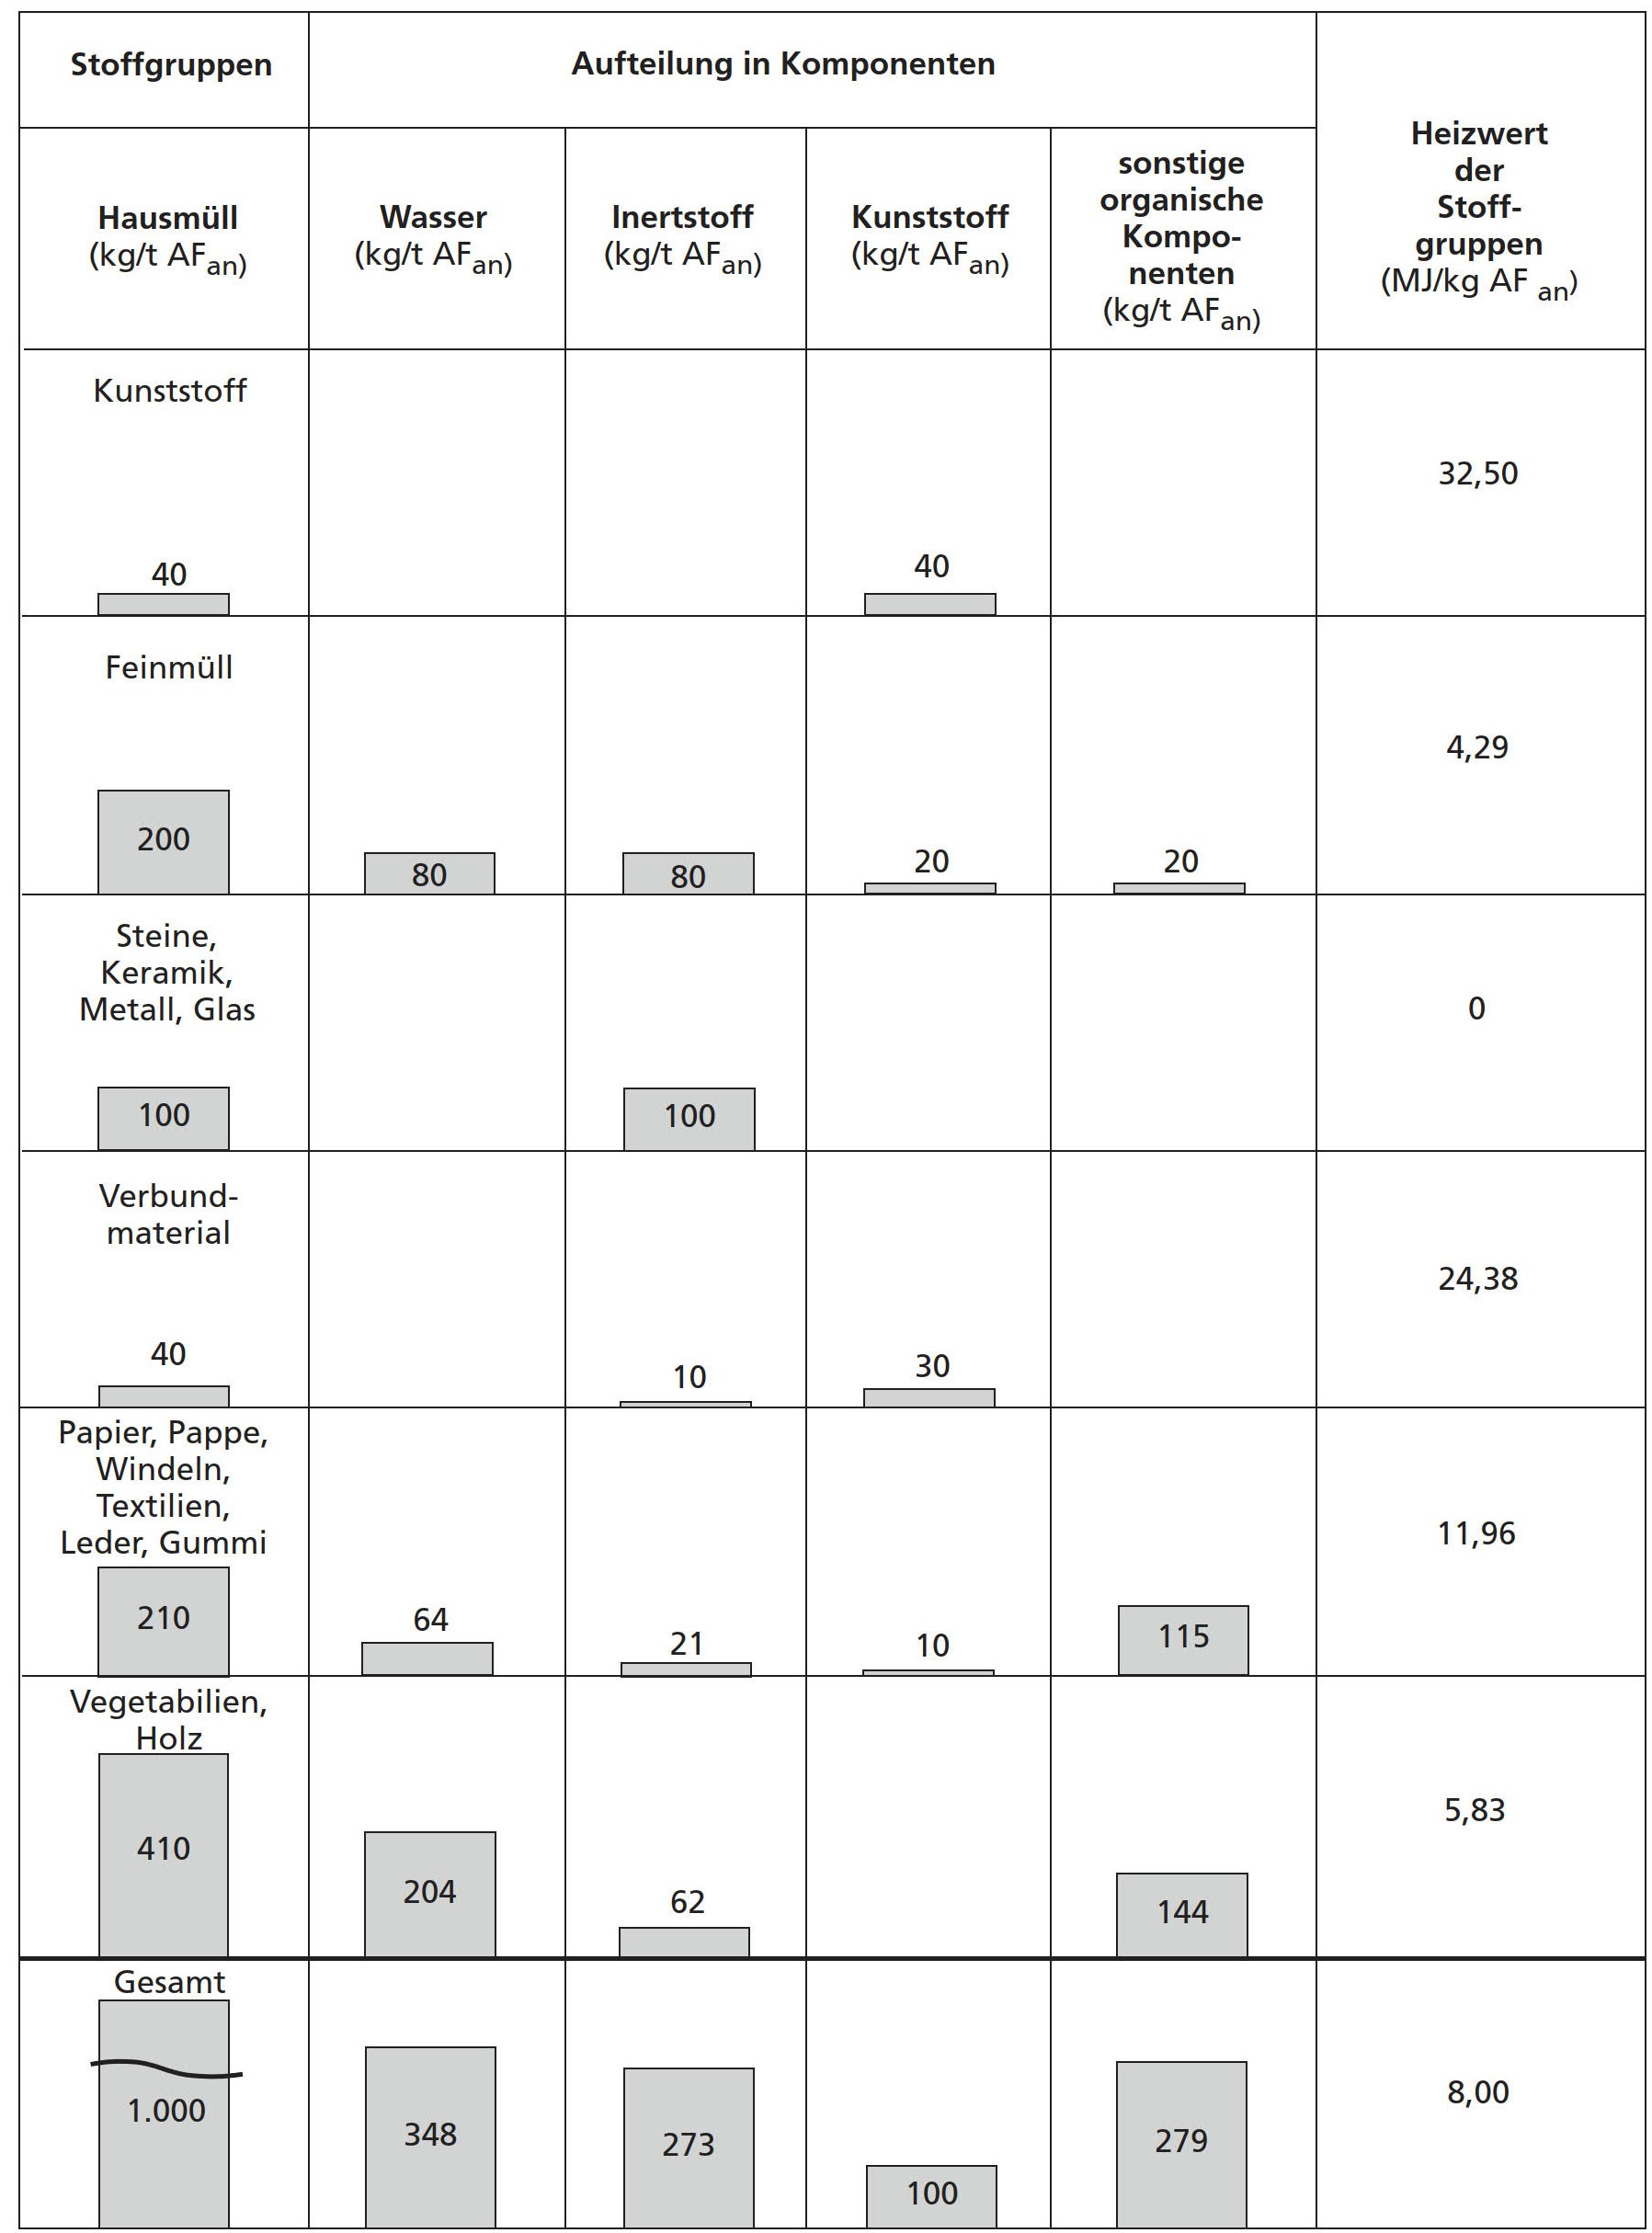
\includegraphics[width=0.90\textwidth]{img/ThermischeVerfahren}
	\caption[Darstellung eines Hausmülls durch unterschiedliche Stoffgruppen und deren Aufteilung auf die Komponenten Wasser, Inertstoff, Kunststoff und sonstigen organischen Komponenten]{Darstellung eines Hausmülls durch unterschiedliche Stoffgruppen und deren Aufteilung auf die Komponenten Wasser, Inertstoff, Kunststoff und sonstigen organischen Komponenten aus \cite[S.23]{scholz2013}}
	\label{fig:ersatzbrennstoffe}
\end{figure}
\FloatBarrier
%Ende

\begin{itemize}	
	\item Plausibilität TS\\ 
	\textcolor{red}{Damit war eher die Trockensubstanz gemeint, wie bei den Berechnungen  unter dem Abschnitt vorher}\\
	\textit{Der Schwefelgehalt des Abfalls setzt sich aus dem Organischen Schwefelgehalt (TOS) und dem Anorganischen Schwefelgehalt(TIS) zusammen. Aus dem Artikel \cite{Schwarzboeck2018} lässt sich ein Referenzwert für den TOS von etwa 8 bis \SI{10}{\gram\per\kilogram} bei Asche- Und Wasserfreiheit ableiten. Das entspricht \SI{0,64}{\mpercent} bis etwa \SI{1}{\mpercent}(siehe Rechnung weiter unten vielleicht noch in den Anhang)
		Schwefelgehalte des Hausmülls schwankten mitte der 1990ger Jahre zwischen \SI{0,3}{\mpercent} und \SI{0,5}{\mpercent} \cite{scholz2013}.}	
\end{itemize}
Der Glühverlust wird im Folgenden indirekt über den Inertstoffgehalt verglichen. Laut der Quelle (siehe Abb. \ref{fig:ersatzbrennstoffe}) besitzt der allgemeine Haushalt einen Inertstoffgehalt von $\approx \SI{27}{\percent}$. Im Vergleich dazu erscheint der Inertstoffgehalt der untersuchten Müllprobe mit $\approx \SI{77}{\percent}$ als hoch bzw. der Glühverlust im Vergleich als niedrig. Die Vermutung, dass die optisch ascheähnlichen Bestandteile tatsächlich intert sind, wäre somit begründet.\\ \\
\textcolor{red}{Muss mal noch schön mit eingebunden bzw. gekürzt werden}\\
\textcolor{blue}{\textit{Das Papier (Illustrationspapier) aus einem Magazin weist eine Glührückstand von ca. \SI{15}{\mpercent} auf \cite{roempppap}. Einige Kunststoffe können theoretisch rückstandsfrei verbrennen. Es besteht also ein enger Bezug zum Füllstoffgehalt. Dieser Füllstoffanteil wurde zuvor schon ausreichend diskutiert. Ein realistischer Mittelwert für den Glührückstand von Kunststoffen wäre wohl \SI{20}{\mpercent}.
Aschegehalte des Hausmülls schwankten mitte der 1990ger Jahre zwischen \SI{25}{\mpercent} und \SI{35}{\mpercent} (siehe Abb. \ref{fig:ersatzbrennstoffe}).
Der im Experiment ermittelte Glührückstand von rund 75\% ist deutlich zu hoch. In der Literatur ist nirgends ein so hoher mineralischer Füllstoffanteil, Glührückstand oder Aschegehalt beschrieben. Es sind 5 wichtige Fehlerquellen zu beachten. Der Müll könnte durch einen beachtlichen mineralischen Feststoffanteil belastet sein. Die Veraschung könnte unvollständig sein, wodurch verbliebene Organische Anteile als anorganisch interpretiert würden. Die Asche könnte bei den angewendeten Temperaturen ihre chemische Zusammensetzung in Anwesenheit von Umgebungsluft verändert haben. Die Asche könnte Feuchtigkeit aus der Umgebungsluft aufgrund ihrer hygroskopischen Eigenschaften angezogen haben. Es könnten Messfehler passiert sein. Bei Vertauschung der Tiegel könnten die Massen falsch subtrahiert worden sein. Dann hätten die Werte aber stark von einander abweichen müssen, weil sich der Fehler für die eine Masse negativ und für die andere Masse positiv ausgewirkt hätte. Letzterer Fehler kann damit ausgeschlossen werden. 
In Anbetracht der vielen möglichen Einflussfaktoren muss der Ermittelte Wert kritisch betrachtet und vorsichtig verwendet werden. Er kann aber nicht als Falsch ausgeschlossen werden.}}
%Tabelle START
\vspace*{-3.5mm}
\renewcommand{\arraystretch}{1.2}
\begin{table}[h!]
	\centering
	\caption[Tabellenausschnitt mit Heizwerten üblicher Brennstoffe]{Tabellenausschnitt mit Heizwerten üblicher Brennstoffe aus \cite{S.Furkus.}}
	\label{tab:heizwerte}
	%\resizebox{10cm}{!}{
	\begin{tabulary}{\textwidth}{C|CC}
		\hline
		\textbf{Energieträger} & \textbf{Heizwert $\boldsymbol{\left[\si{\kWh\per\kg}\right]}$} & \textbf{Brennwert $\boldsymbol{\left[\si{\kWh\per\kg}\right]}$} \\ 
		\hline
		Stadtgas			&	6,8...8,7	&	7,7...9,8\\
		Benzin				&	12,11	&	13,06\\
		Waldfrisches Holz	&	1,90	&	k.A.\\
		Hackschnitzel		&	3,5...4,0	&	3,8...4,3\\
		Papier 				& 	4,17 	&	k.A. \\	
		Hausmüll			&	2,78	&	k.A.\\
		\hline
	\end{tabulary}
	%}
\end{table}
\FloatBarrier
\vspace*{-2.5mm}
%Tabelle Ende

Der Brennwert ist, richtiger Weise, höher als der Heizwert, da die im Wasserdampf gebundene Energie mit folgender Kondensation betrachtet wird. Ein Gemisch  welches zu gleichen Teilen aus Haus- und Papiermüll besteht hat etwa einen Heizwert von \SI{3,5}{\kilo\watt\hour\per\kilogram} oder \SI{12,6}{\mega\joule\per\kilogram} (siehe Tab. \ref{tab:heizwerte}). Mit \SI{1,65}{\kWh\per\kg} ist der berechnete Brennwert etwa halb so groß. Verglichen mit üblichen Brennstoffen aus Tab. \ref{tab:heizwerte} zeigt sich die Müllprobe als Ersatzbrennstoff mit \SI{1,65}{\kWh\per\kg} schlechter als die angegebenen Brennwerte für Benzin, Stadtgas und Hackschnitzel. Das erscheint sinnvoll durch den hohen Inertstoffgehalt, da dadurch pro Kilogramm weniger Energie durch Verbrennung frei werden kann. Für weitere Vergleiche wird Bezug auf den Heizwert genommen, da hierfür mehr Angaben aus Tab. \ref{tab:heizwerte} zu entnehmen sind.\\ 
Der Heizwert der Probe siedelt sich mit $\approx \SI{5}{\mega \joule \per \kg}$ bzw. $\approx \SI{1,5}{\kWh\per\kg}$ vergleichsweise zwischen die Müllfraktionen von Feinmüll mit $\approx \SI{4,29}{\mega \joule \per \kg}$ und Holz, Vegetablien mit $\approx \SI{5,83}{\mega \joule \per \kg}$ an (siehe Tab. \ref{fig:ersatzbrennstoffe}). Aus rein optischer Einschätzung scheint lediglich der Feinmüll als plausibel, da Holz bzw. Vegetabilien nicht vorrangig zu erkennen sind. Die untersuchte Müllprobe liegt somit unter dem Heizwert für allgemeinen Hausmüll mit $\approx \SI{8,00}{\mega \joule \per \kg}$ (siehe Tab. \ref{fig:ersatzbrennstoffe}). Das wiederum erscheint durch den hohen Inertstoffgehalt als sinnvoll, nimmt man den Messwert der Müllfraktion von Papier, Pappe, etc. $\approx \SI{11,96}{\mega \joule \per \kg}$ in die Betrachtung des Heizwertes als Bestandteil hinzu (siehe Tab. \ref{fig:ersatzbrennstoffe}). Aufgrund der unterschiedlichen Zusammensetzungen von Müllproben erscheint eine genauere Plausibilitätsbetrachtung als schwierig. Die Dimensionen dieser Müllprobe scheinen, was den Heizwert anbelangt, jedoch nicht unrealistisch zu sein.\\
Ausgehend von der Sinnhaftigkeit der erhobenen Daten lässt der Heizwert, ähnlich wie der Brennwert, ebenfalls mit Heizwerten von üblichen Brennstoffen der Tabelle \ref{tab:heizwerte} vergleichen. Die Probe schneidet im Vergleich auch in Bezug auf mehr Energieträger deutlich schlechter ab. Lediglich waldfrisches Holz, mit \SI{1,90}{\kWh\per\kg} Heizwert, ist an dieser Stelle annähernd vergleichbar. Somit wird auch durch den Heizwertvergleich deutlich, dass sich die Müllprobe selbst vergleichsweise schlecht als Ersatzbrennstoff eignet. Begründung liegt auch hier wieder im hohen Inertstoffgehalt, welcher keinen energetischen Nutzen darstellt.\\
Um energetisch hochwertigere Brenn- bzw. Heizwerte zu erzielen, könnte untersucht werden ob eine Reduzierung des Inertstoffgehaltes pro Kilogramm, durch feineres Sieben der Müllprobe, zielführend ist.\\ \\
Zusammenfassend lässt sich sagen, dass lediglich Aussagen zur qualitativen Beschaffenheit getroffen können, da die Zusammensetzung der Müllprobe nicht genauer bestimmt ist. Ein Widerspruch ist hier nicht zu erkennen, da die Brenn- bzw. Heizwertewerte zwar im Vergleich zu anderen Energieträgern gering, aber immerhin in der selben Größenordnung liegen.\linebreak
Erwartungsgemäß ist der Heizwert geringer als der Brennwert da die latente Wärme des Wasserdampfes in diesem nicht verwertet wird.\\
%===========================================
%Optional Berechnung zum Schwefelgehalt.

%	Eine Beladung von 8 - 10g/kg mit Schwefel bei Asche und Wasserfreiheit
%	\begin{flalign}
%	\frac{10 g}{1000 g} &= 1\%\\
%	\frac{8 g}{1000 g} &= 0,8\%
%	\end{flalign}
%	Angleichung an reale Verhältnisse durch Annahme von maximal 20 ma\% Asche und 5\% Wasser.
%	\begin{flalign}
%	\frac{10 g}{1250 g} &= 0,8\%\\
%	\frac{8 g}{1250 g} &= 0,64\%
%	\end{flalign}
%=============================================
\textcolor{red}{Da fehlt noch ein bisschen was}\\
Der Chlorgehalt könnte zwischen etwa \SI{0,3}{\mpercent} und \SI{3}{\mpercent} \cite{LLA_Abfallanalyse}. Chlorgehalte des Hausmülls schwankten mitte der 1990ger Jahre zwischen \SI{0,4}{\mpercent} und \SI{1}{\mpercent} \cite{scholz2013}.
Das Papier (Illustrationspapier) aus einem Magazin weist eine Glührückstand von ca. \SI{15}{\mpercent} auf \cite{roempppap}. Einige Kunststoffe können theoretisch rückstandsfrei verbrennen. Es besteht also ein enger Bezug zum Füllstoffgehalt. Dieser Füllstoffanteil wurde zuvor schon ausreichend diskutiert. Ein realistischer Mittelwert für den Glührückstand von Kunststoffen wäre wohl \SI{20}{\mpercent}.
Aschegehalte des Hausmülls schwankten mitte der 1990ger Jahre zwischen \SI{25}{\mpercent} und \SI{35}{\mpercent} \cite{scholz2013}.
Der im Experiment ermittelte Glührückstand von rund 75\% ist deutlich zu hoch. In der Literatur ist nirgends ein so hoher mineralischer Füllstoffanteil, Glührückstand oder Aschegehalt beschrieben. Es sind 5 wichtige Fehlerquellen zu beachten. Der Müll könnte durch einen beachtlichen mineralischen Feststoffanteil belastet sein. Die Veraschung könnte unvollständig sein, wodurch verbliebene Organische Anteile als anorganisch interpretiert würden. Die Asche könnte bei den angewendeten Temperaturen ihre chemische Zusammensetzung in Anwesenheit von Umgebungsluft verändert haben. Die Asche könnte Feuchtigkeit aus der Umgebungsluft aufgrund ihrer hygroskopischen Eigenschaften angezogen haben. Es könnten Messfehler passiert sein. Bei Vertauschung der Tiegel könnten die Massen falsch subtrahiert worden sein. Dann hätten die Werte aber stark von einander abweichen müssen, weil sich der Fehler für die eine Masse negativ und für die andere Masse positiv ausgewirkt hätte. Letzterer Fehler kann damit ausgeschlossen werden. 
In Anbetracht der vielen möglichen Einflussfaktoren muss der Ermittelte Wert kritisch betrachtet und vorsichtig verwendet werden. Er kann aber nicht als Falsch ausgeschlossen werden.
%\begin{tikzpicture}
%\begin{axis}[
%xbar=1pt,% space of 0pt between adjacent bars
%bar width=11,
%width=15cm,
%height=11cm,
%%minor y tick num=4,
%xmax=40,xmin=-40,
%x tick label style={/pgf/number format/.cd,%
%	scaled x ticks = false,
%	set decimal separator={,},
%	fixed},
%symbolic y coords={Zn,Cl,Mn,Uub,As},
%ytick=data,
%xtick={-30.5,-20.5,-10.5,0,10.5,20.5,30.5},
%grid=major,
%%enlargelimits=0.15,
%]
%\addplot coordinates {
%	(-10.3,Mn) (15.4,Cl) (5,Zn) (24,Uub) (30,As)
%};
%\addplot coordinates {
%	(-3,Mn) (5,Cl) (15,Zn) (20,Uub) (35,As)
%};
%\addplot coordinates {
%	(-8,Mn) (-19,Cl) (20,Zn) (30,Uub) (5,As)
%};
%
%\end{axis}
%\end{tikzpicture}


